\documentclass[border=10pt]{standalone}
\usepackage{pgfplots}
\pgfplotsset{compat=1.18}

\begin{document}
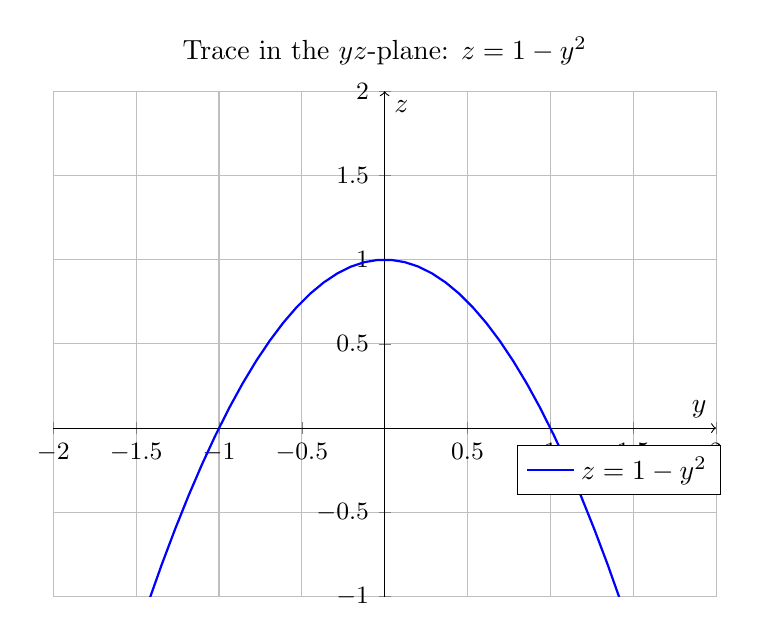
\begin{tikzpicture}
\begin{axis}[
    xlabel={$y$},
    ylabel={$z$},
    title={Trace in the $yz$-plane: $z = 1 - y^2$},
    domain=-2:2,
    samples=50,
    grid=major,
    width=10cm,
    height=8cm,
    ymin=-1,
    ymax=2,
    xmin=-2,
    xmax=2,
    axis lines=center,
    axis line style={->},
    ticklabel style={font=\small},
    legend style={at={(0.7,0.3)},anchor=north west}
]
\addplot[blue, thick] {1 - x^2};
\legend{$z = 1 - y^2$}
\end{axis}
\end{tikzpicture}
\end{document}